\chapter{Exploitation}
\markboth{Exploitation}{}

Adesso che sono state ottenute abbastanza informazioni sulla macchina, si può procedere con la fase di \emph{Exploitation}

\section{Strategie Automatizzate}
Il primo passo eseguito è stato quello di verificare effettivamente quali potevano essere le vulnerabilità sfruttabili consultando tutti i report ottenuti dai tool e, effettivamente, le strade più promettenti sono:
\begin{enumerate}
    \item Sfruttamento della vulnerabilità di \textbf{SQL Injection};
    \item Sfruttamento della vulnerabilità di \textbf{mod\_ssl};
    \item Sfruttamento della vulnerabilità di \textbf{ProFTPD};
    \item Sfruttamento della vulnerabilità \textbf{HeartBleed};
    \item Sfruttamento di vulnerabilità di \textbf{phpMyAdmin}
\end{enumerate}

\subsection{Utilizzo di \texttt{sqlmap}}
Per tentare di sfruttare la vulnerabilità di \textbf{SQL Injection} sull'asset si è deciso di utilizzare \texttt{sqlmap}, uno strumento molto potente e in grado di automatizzare il processo di \emph{injection} sulle pagine. Per avviarlo basta eseguire il comando:
\begin{lstlisting}[language=bash]
    sqlmap -u https://10.0.2.4 -a -forms
\end{lstlisting}
dove con \texttt{-u} si specifica l'indirizzo target, con \texttt{-a} si specifica l'intenzione di voler recuperare tutto il possibile (schemi, tabelle, ecc.) e con \texttt{-forms} si specifica l'intenzione di sfruttare i \emph{form} presenti nella pagina.

Eseguendo \texttt{sqlmap} sulle varie pagine dell'asset, i risultati sono i seguenti:
\begin{figure}[h]
    \begin{subfigure}{0.5\textwidth}
        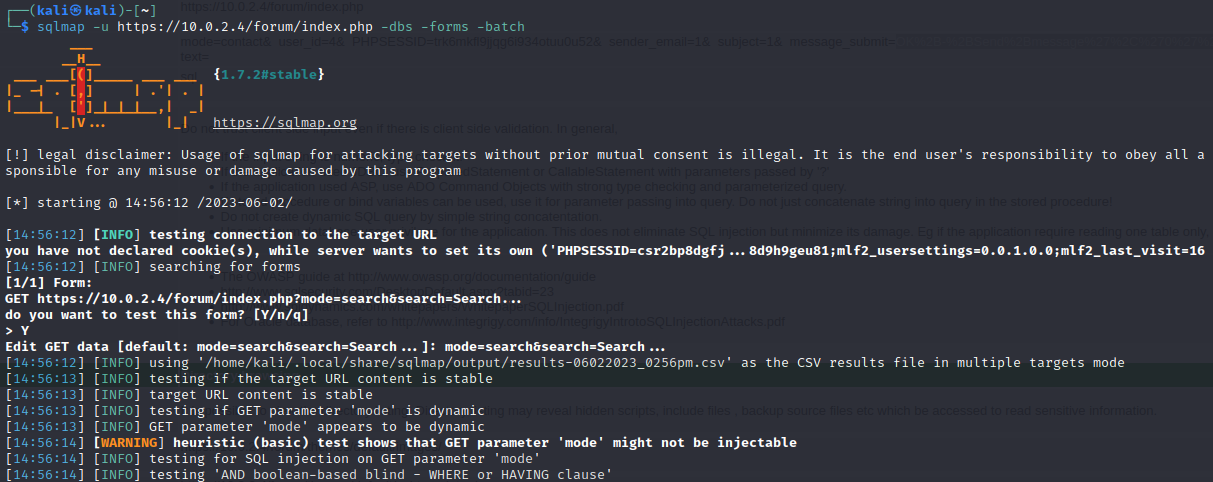
\includegraphics[width=1\textwidth]{capitoli/figure/sqlmap-forum-index-1.png}
        \caption{Prima parte del risultato parziale di \texttt{sqlmap}\\ su \emph{forum/index.php}}
        \label{fig:sqlmap-forum-index-1}
    \end{subfigure}
    \begin{subfigure}{0.5\textwidth}
        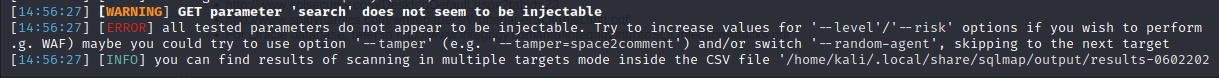
\includegraphics[width=1\textwidth]{capitoli/figure/sqlmap-forum-index-2.png}
        \caption{Seconda parte del risultato parziale di \texttt{sqlmap} su \emph{forum/index.php}}
        \label{fig:sqlmap-forum-index-2}
    \end{subfigure}
    \begin{subfigure}{0.5\textwidth}
        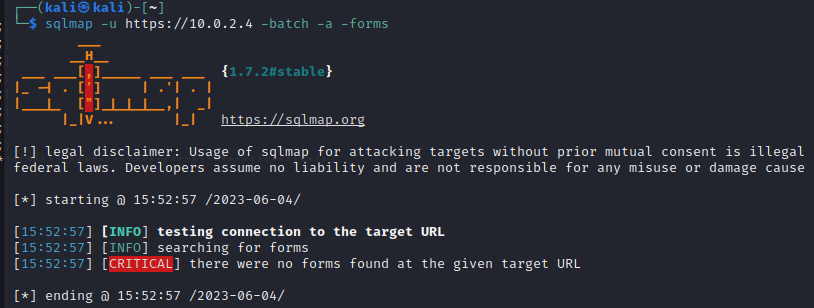
\includegraphics[width=1\textwidth]{capitoli/figure/sqlmap-index.png}
        \caption{Risultato di \texttt{sqlmap} su \emph{index.html}}
        \label{fig:sqlmap-index}
    \end{subfigure}
    \begin{subfigure}{0.5\textwidth}
        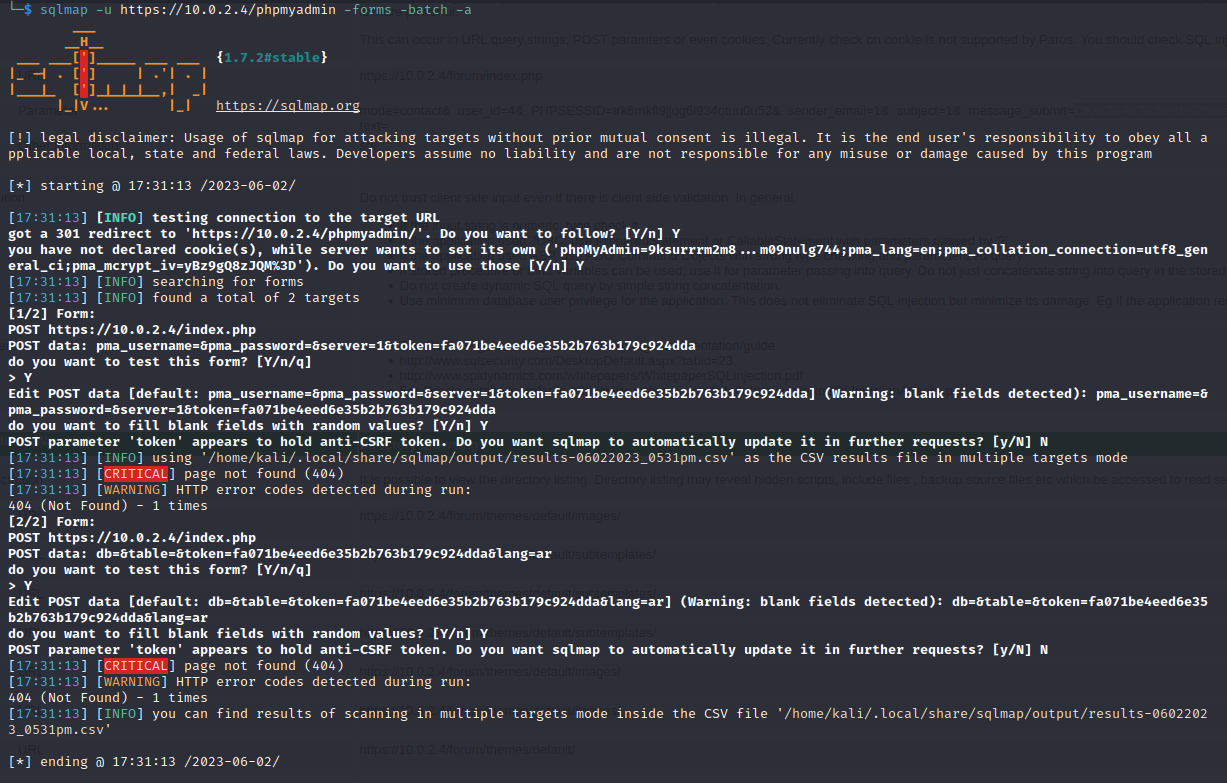
\includegraphics[width=1\textwidth]{capitoli/figure/sqlmap-phpmyadmin.png}
        \caption{Risultato di \texttt{sqlmap} su \emph{phpmyadmin}}
        \label{fig:sqlmap-phpmyadmin}
    \end{subfigure}
    \caption{Risultati ottenuti con \texttt{sqlmap}}
    \label{fig:sqlmap}
\end{figure}

Come si può notare dalle varie esecuzioni di \texttt{sqlmap} possiamo stabilire che purtroppo lo sfruttamento della \textbf{SQL Injection} non è praticabile e non permette di ottenere ulteriori informazioni. A questo punto, ciò che si può supporre è che il rilevamento effettuato da \texttt{paros} e da \emph{Nessus} non è altro che un falso positivo.

In vista dei risultati ottenuti, quindi, si può scartare questa strategia e procedere con le successive.

\subsection{Utilizzo della suite \emph{Metasploit}}
Il passo successivo è quello di cercare di sfruttare le altre vulnerabilità rilevate riguardo \textbf{mod\_ssl, ProFTPD} e \textbf{HeartBleed}. Utilizzando la suite \emph{Metasploit}, quello che si può fare è cercare degli \emph{exploit} in grado di sfruttare una delle vulnerabilità rilevate dai tool utilizzati per la scansione. Per eseguire la ricerca viene quindi lanciata la console di \emph{Metasploit} con il comando \texttt{msfconsole} e successivamente viene utilizzato il comando \texttt{search}.\\
La prima ricerca effettuata riguarda \textbf{mod\_ssl} che, a quanto rivelato dal report, una versione deprecata di questo strumento potrebbe permettere addirittura l'esecuzione di codice arbitrario da remoto. Tuttavia, effettuando la ricerca non viene trovato nulla a riguardo, come mostrato di seguito:
\begin{figure}[h]
    \centering
    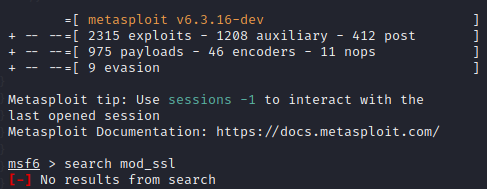
\includegraphics[width=0.5\textwidth]{capitoli/figure/metasploit-mod_ssl.png}
    \caption{Risultato ricerca di \textbf{mod\_ssl}}
    \label{fig:metasploit-modssl}
\end{figure}

Anche effettuando una ricerca sul sito del \emph{MITRE} si scopre che, nonostante questa possibilità, non sono forniti exploit a riguardo.\\
Allora quello che si può fare è continuare la ricerca con \textbf{ProFTPD} e, questa volta, otteniamo dei risultati come mostrato di seguito:
\begin{figure}[h]
    \centering
    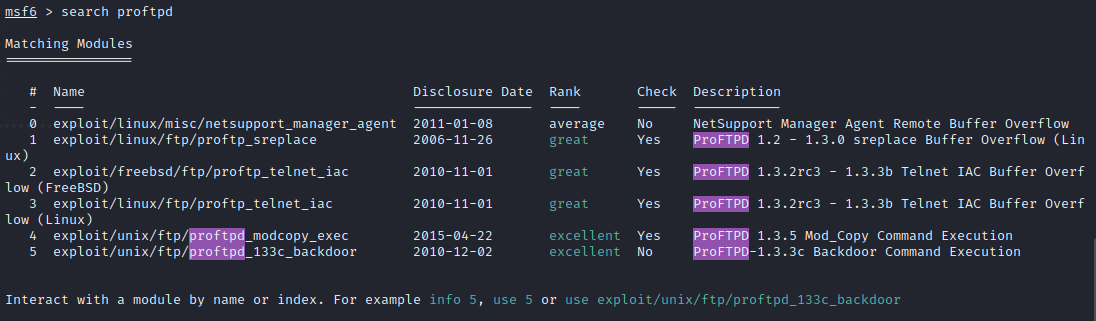
\includegraphics[width=0.6\textwidth]{capitoli/figure/metasploit-proftpd.png}
    \caption{Risultato ricerca di \textbf{ProFTPD}}
    \label{fig:metasploit-proftpd}
\end{figure}

Tenendo presente che la versione di \textbf{ProFTPD} installata è \textbf{1.3.4a}, si nota che solo un exploit potrebbe essere utilizzabile in quanto gli altri sono efficaci solo contro versioni precedenti a quella installata. L'exploit in questione è \textbf{modcopy\_exec} che permette la copia di qualunque file accessibile con i permessi dell'utente che esegue il servizio \textbf{ProFTPD} e anche esecuzione di codice tramite \emph{PHP}\cite{proftpd-mod-copy}.

Selezionando questo exploit e come payload una reverse shell con \emph{netcat} (con le opportune configurazioni),  il risultato è che non abbiamo successo poichè probabilmente non si hanno i permessi di scrittura sulla cartella target, come mostrato di seugito:
\begin{figure}[h]
    \centering
    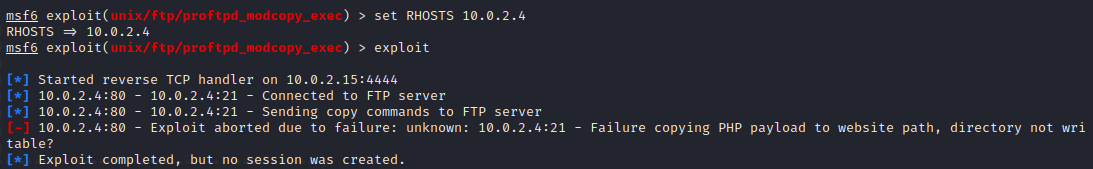
\includegraphics[width=0.5\textwidth]{capitoli/figure/metasploit-proftpd-attack.png}
    \caption{Risultato attacco di \textbf{ProFTPD}}
    \label{fig:metasploit-proftpd-attack}
\end{figure}

Lo stesso risultato è ottenuto anche con tutti gli altri payload, sia di tipo reverse che di tipo bind, rendendo anche questa strada non utilizzabile.\\
Rimossa anche quest'altra strada, un ulteriore tentativo è quello di sfruttare \textbf{HeartBleed}. Come fatto in precedenza, viene effettuata la ricerca di exploit a riguardo e il risultato è il seguente:
\begin{figure}[h]
    \centering
    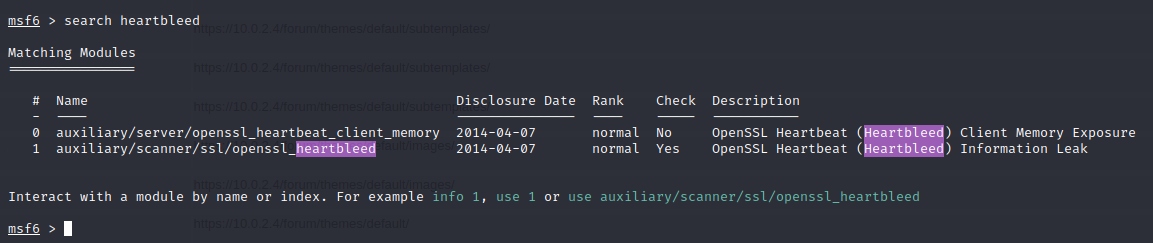
\includegraphics[width=0.7\textwidth]{capitoli/figure/metasploit-heartbleed-list.png}
    \caption{Risultato ricerca di \textbf{HeartBleed}}
    \label{fig:metasploit-heartbleed}
\end{figure}

Non è stato trovato un exploit a riguardo ma un modulo ausiliario, il quale non permette di ottenere una \emph{shell} (quindi il controllo della macchina), ma permette l'ottenimento di altre informazioni che possono tornare molto utili. Se ad esempio si riuscisse a sfruttare questa vulnerabilità, si potrebbero persino ottenere password e chiavi private salvate sul server. Utilizzando lo scanner, tuttavia, il risultato è che ancora una volta non si riesce ad ottenere nulla, come mostrato di seguito:
\begin{figure}[h]
    \centering
    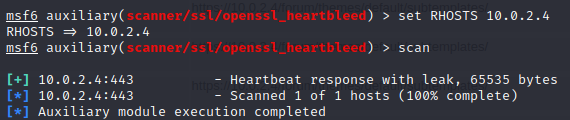
\includegraphics[width=0.6\textwidth]{capitoli/figure/metasploit-heartbleed-scan.png}
    \caption{Risultato attacco con \textbf{HeartBleed}}
    \label{fig:metasploit-heartbleed-attack}
\end{figure}

Infatti l'esecuzione del modulo termina senza ottenere nulla, confermando però la presenza della vulnerabilità \textbf{HeartBleed}.\\
A questo punto non resta che sperare in qualche vulnerabilità di \textbf{phpMyAdmin} (visto che era stata rilevato un falso positivo) e, effettuando una ricerca, si ottengono i seguenti risultati:
\begin{figure}[h]
    \centering
    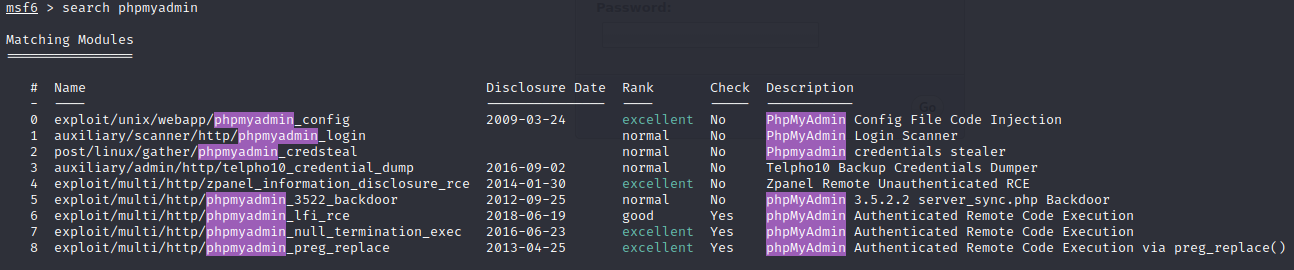
\includegraphics[width=0.7\textwidth]{capitoli/figure/metasploit-phpmyadmin.png}
    \caption{Risultato ricerca di \textbf{phpMyAdmin}}
    \label{fig:metasploit-phpmyadmin}
\end{figure}

Escludendo i moduli \emph{post} (Utilizzabili dopo aver eseguito l'exploitation con successo) e \emph{auxiliary}, gli unici \emph{exploit} interessanti sono gli ultimi 3. Sfortunatamente, dopo l'esecuzione di tutti i payload di tutti e 3 gli exploit, non è stato possibile eseguire l'exploiting della macchina \emph{10.0.2.4}, come mostrato parzialmente di seguito:
\begin{figure}[h]
    \centering
    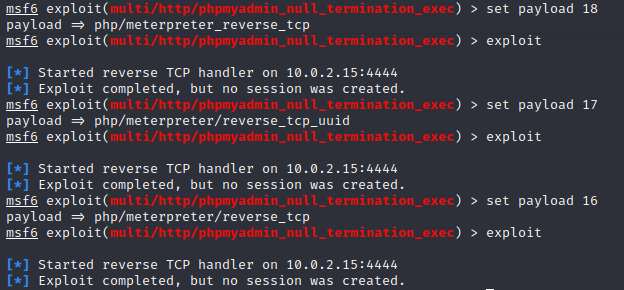
\includegraphics[width=0.7\textwidth]{capitoli/figure/metasploit-phpmyadmin-attack.png}
    \caption{Risultato parziale dell'attacco a \textbf{phpMyAdmin}}
    \label{fig:metasploit-phpmyadmin-attack}
\end{figure}

Purtroppo, dopo quest'ultimo fallimento, non sembrano esserci altre vie percorribili basandosi sulle informazioni acquisite in precedenza.

\subsection{Utilizzo della GUI \emph{Armitage}}
Un ultimo tentativo che è possibile realizzare è quello di utlizzare \emph{Armitage}, una GUI per la suite \emph{Metasploit}. Il motivo è per utilizzare una funzione offerta chiamata \textbf{Hail Mary}, che si occupa di effettuare il bruteforce di tutti gli exploit e payload compatibili su una macchina target nella speranza di instaurare almeno una \emph{sessione}. Per utilizzare la funzione precedentemente citata, bisogna effettuare di nuovo le fasi target discovery ed enumeration all'interno di \emph{Armitage} e, una volta finite, basta utilizzare l'opzione \emph{find attacks} per filtrare gli exploit che sono compatibili con la macchina target. Il risultato ottenuto fino a questo momento è il seguente:
\begin{figure}[h]
    \centering
    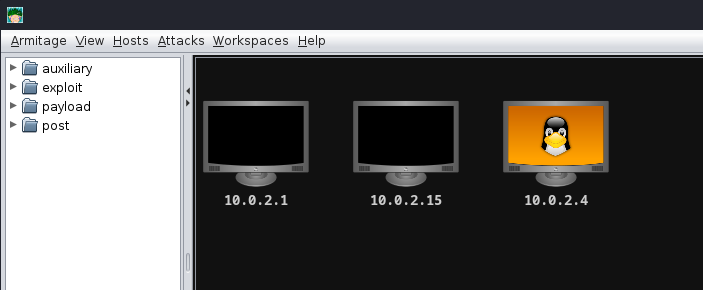
\includegraphics[width=0.7\textwidth]{capitoli/figure/armitage.png}
    \caption{Output di \emph{Armitage} dopo le scansioni}
    \label{fig:armitage}
\end{figure}

A questo punto è possibile lanciare la funzione \emph{Hail Mary} e, dopo aver atteso che tutti gli exploit siano stati lanciati, si può osservare che anche con questa strategia \emph{estrema} non è stato possibile avere accesso alla macchina. Un report con gli exploit lanciati da questa funzione è consultabile nella cartella \emph{Report} con il nome \textbf{armitage-hailmary.log}.

\subsection{Fallimento delle strategie automatizzate}
Nonostante i report fossero promettenti inizialmente, visto che sono state trovate trovate vulnerabilità interessanti, l'utilizzo di strumenti automatici per l'exploitation non ha mostrato i risultati sperati e si è rivelato un completo fallimento. Una possibile ragione per cui questo è accaduto può essere il fatto che l'asset da attaccare in realtà è una macchina che non è stata pensata per un \emph{Penetration Testing} ma bensì per una \emph{sfida CTF}. Questo significa, quindi, che la macchina non è stata realizzata utilizzando servizi vulnerabili (sarebbe stata facilitata la risoluzione della \emph{sfida CTF}) ma utilizzando servizi "aggiornati" (ovviamente in riferimento alle versioni dell'anno di rilascio) che non presentano vulnerabilità tali da fornire accesso completo o parziale alla macchina e navigazione libera del file system della macchina.\\
In base a questa osservazione non ci sono quindi altri modi per avere accesso alla macchina se non quello di risolvere la sfida interrogando manualmente la macchina ed estrapolando le informazioni fornite dai servizi offerti.

\section{Strategie manuali}
La decisione presa, a questo punto, è quella di procedere con l'analisi manuale dell'asset.
\subsection{Visita del server web}

\subsection{Accesso al servizio \emph{FTP}}

\subsection{Analisi della pagina forum}

\subsection{Compromissione di un utente del forum}

\subsection{Compromissione di \textbf{phpmyadmin}}

\subsection{Cracking degli hash ottenuti}

\subsection{Accesso al servizio FTP come nuovo utente}

\subsection{Ottenimento di una shell}